\section{Root Finding}
    \begin{figure}[H]
        \centering
        \captionsetup{type=figure}
        \resizebox{\textwidth}{!}{%
            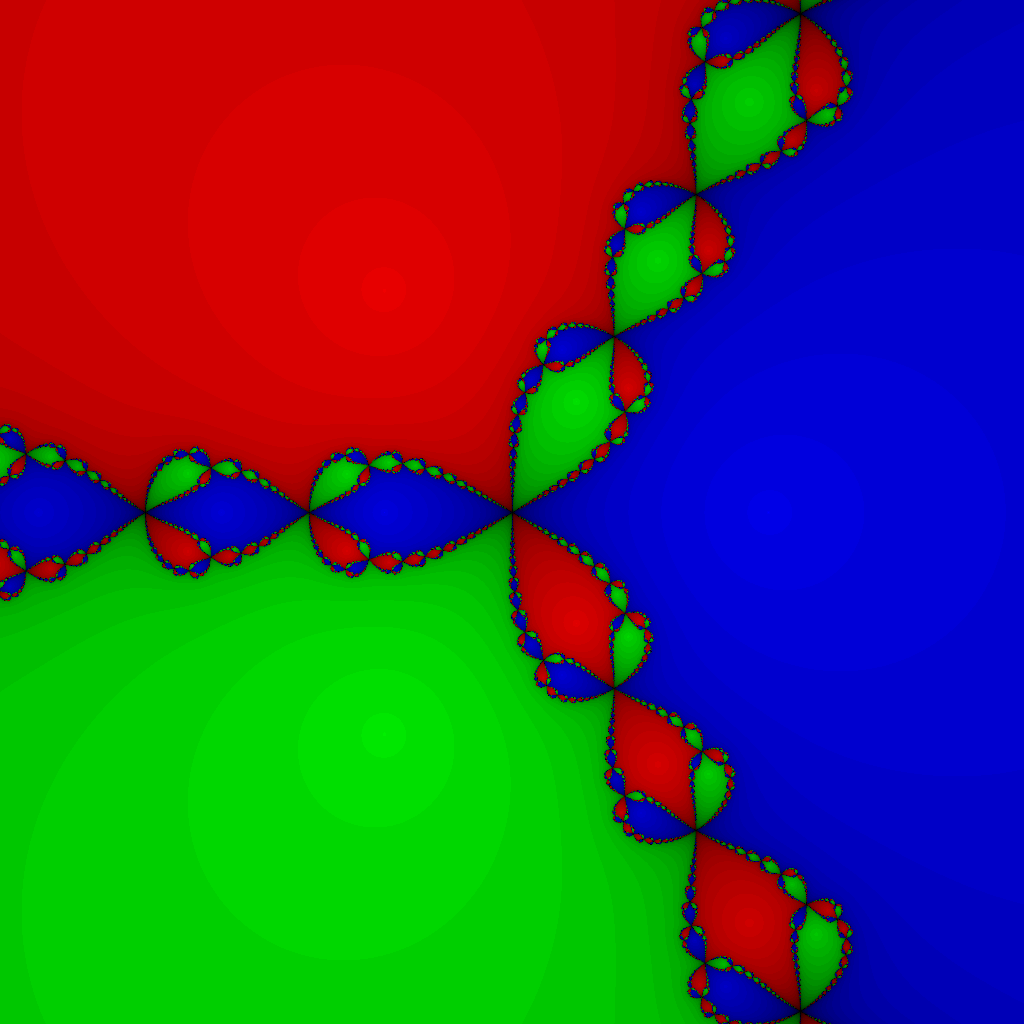
\includegraphics{newton_fractal_z_cubed_minus_one.png}
        }
        \caption{Newton Fractal for $z^{3}-1=0$}
        \label{fig:Diff_Theory_Newton_Fractal}
    \end{figure}
    The Python code used to generated this is given below.
    It can be altered to try various functions, and this
    is encouraged.
    \newpage
    \begin{lstlisting}[%
        language=python,
        basicstyle=\footnotesize\ttfamily,
        frame=single,
        gobble=16
    ]
        from PIL import Image
        import numpy as np

        # Set range for x and y axes.
        x_min, x_max = -1.0, 1.0
        y_min, y_max = -1.0, 1.0

        # Colors for the roots (Red, Green, Blue).
        colors = [(255, 0, 30), (0, 255, 30), (0, 30, 255)]

        size = 1024
        img = Image.new("RGB", (size, size), (255, 255, 255))

        # List the roots of z^3-1
        roots = [1.0+0.0j, -0.5+0.8660254037844386j, -0.5-0.8660254037844386j]
        roots = np.array(roots)
        for y in range(size):
            z_y = y * (y_max - y_min)/(size - 1) + y_min
            for x in range(size):
                z_x = x * (x_max - x_min)/(size - 1) + x_min
                z = complex(z_x, z_y)

                # Allow 40 iterations for Newton-Raphson.
                for iters in range(40):
                    # Perfrom Newton-Raphson on z^3 - 1 (Simplifying as well).
                    root = (2.0*z*z*z + 1)/(3.0*z*z)

                    # Checks for convergence
                    if abs(root - z) < 10e-10:
                        break
                    z = root

                ind = np.min((
                    np.abs(root-roots) == np.min(np.abs(root-roots))
                ).nonzero())
                col = colors[ind]
                col = [k for k in col]

                # Create a gradient in color to emphasize rate of convergence.
                col[ind] -= 10*iters
                col = tuple([k for k in col])
                img.putpixel((x, y), col)
        img.save("NewtonRoots.png", "PNG")
    \end{lstlisting}
